\documentclass[margin=0mm]{standalone}
\usepackage{tikz}
\usepackage{pgfplots}
 \pgfplotsset{compat=newest}

\usepgfplotslibrary{fillbetween}

\usetikzlibrary{calc}

\begin{document}


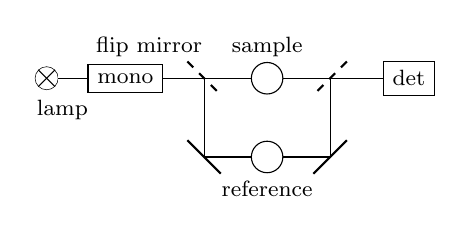
\begin{tikzpicture}[font=\footnotesize]
%\useasboundingbox (0,0) rectangle (5,5);
%\draw (0,0) rectangle (5,5);


\coordinate (lamp) at (0,0);
\coordinate (mono) at ($(lamp) + (1,0)$);
\coordinate (bs1) at ($(mono) + (1,0)$);
\coordinate (sample) at ($(bs1) + (0.8,0)$);
\coordinate (bs2) at ($(sample) + (0.8,0)$);
\coordinate (det) at ($(bs2) + (1,0)$);

\coordinate (ref) at ($(sample) + (0,-1)$);
\coordinate (m1) at ($(bs1) + (0,-1)$);
\coordinate (m2) at ($(bs2) + (0,-1)$);


\draw (lamp.west) -- (det.east);
\draw (bs1) -- (m1) -- (m2) -- (bs2);


\begin{scope}
    \clip (0, 0) circle (1.5mm);
   \draw[fill=white]  (lamp) circle (1.5mm);
  \draw (-1,-1) -- (1,1);
  \draw (-1,1) -- (1,-1);
  \end{scope}


\node[rectangle, draw, fill=white] at (mono) {mono} ;
\draw [dashed, thick] ($(bs1) + (135:3mm)$) -- ++(-45:6mm) ;

\draw [fill=white] (sample) circle (2mm);
\draw [dashed, thick] ($(bs2) + (45:3mm)$) -- ++(-135:6mm) ;

\node[rectangle, draw, fill=white]  at (det) {det} ;

\draw [fill=white] (ref) circle (2mm);
\draw [solid, thick] ($(m1) + (135:3mm)$) -- ++(-45:6mm) ;
\draw [solid, thick] ($(m2) + (45:3mm)$) -- ++(-135:6mm) ;

\node at (lamp) [yshift=-4mm, xshift=2mm] {lamp};
\node at (sample) [yshift=+4mm] {sample};
\node at (ref) [yshift=-4mm] {reference};
\node at (bs1) [yshift=4mm, xshift=-7mm]{flip mirror};

\end{tikzpicture}


\end{document}